% =====================================================================
% Chapter 4: System Design and Implementation
% =====================================================================
\chapter{System Design and Implementation}
\label{ch:system-design}

\section{Overview}

The complete system developed in this thesis consists of two independent
but conceptually related pipelines: an \textbf{image-based pipeline} for
the SoccerNet SN-Jersey dataset, and a \textbf{video-based pipeline} for
broadcast football clips. This chapter presents the architecture and
workflow of each pipeline, including flow diagrams, module
responsibilities, and the data artefacts produced at each stage.

\section{Image-Based Pipeline}
\label{sec:image-pipeline}

\subsection{High-Level Workflow}

The image pipeline transforms a curated list of SoccerNet player-image
paths into a per-image, per-player CSV manifest containing predicted and
ground-truth jersey numbers, OCR confidences, and intermediate diagnostic
fields. Figure~\ref{fig:pipeline-reference} illustrates the end-to-end
pipeline in a compact reference-style overview, showing each processing
stage and the data artefacts it produces.

\begin{figure}[H]
    \centering
    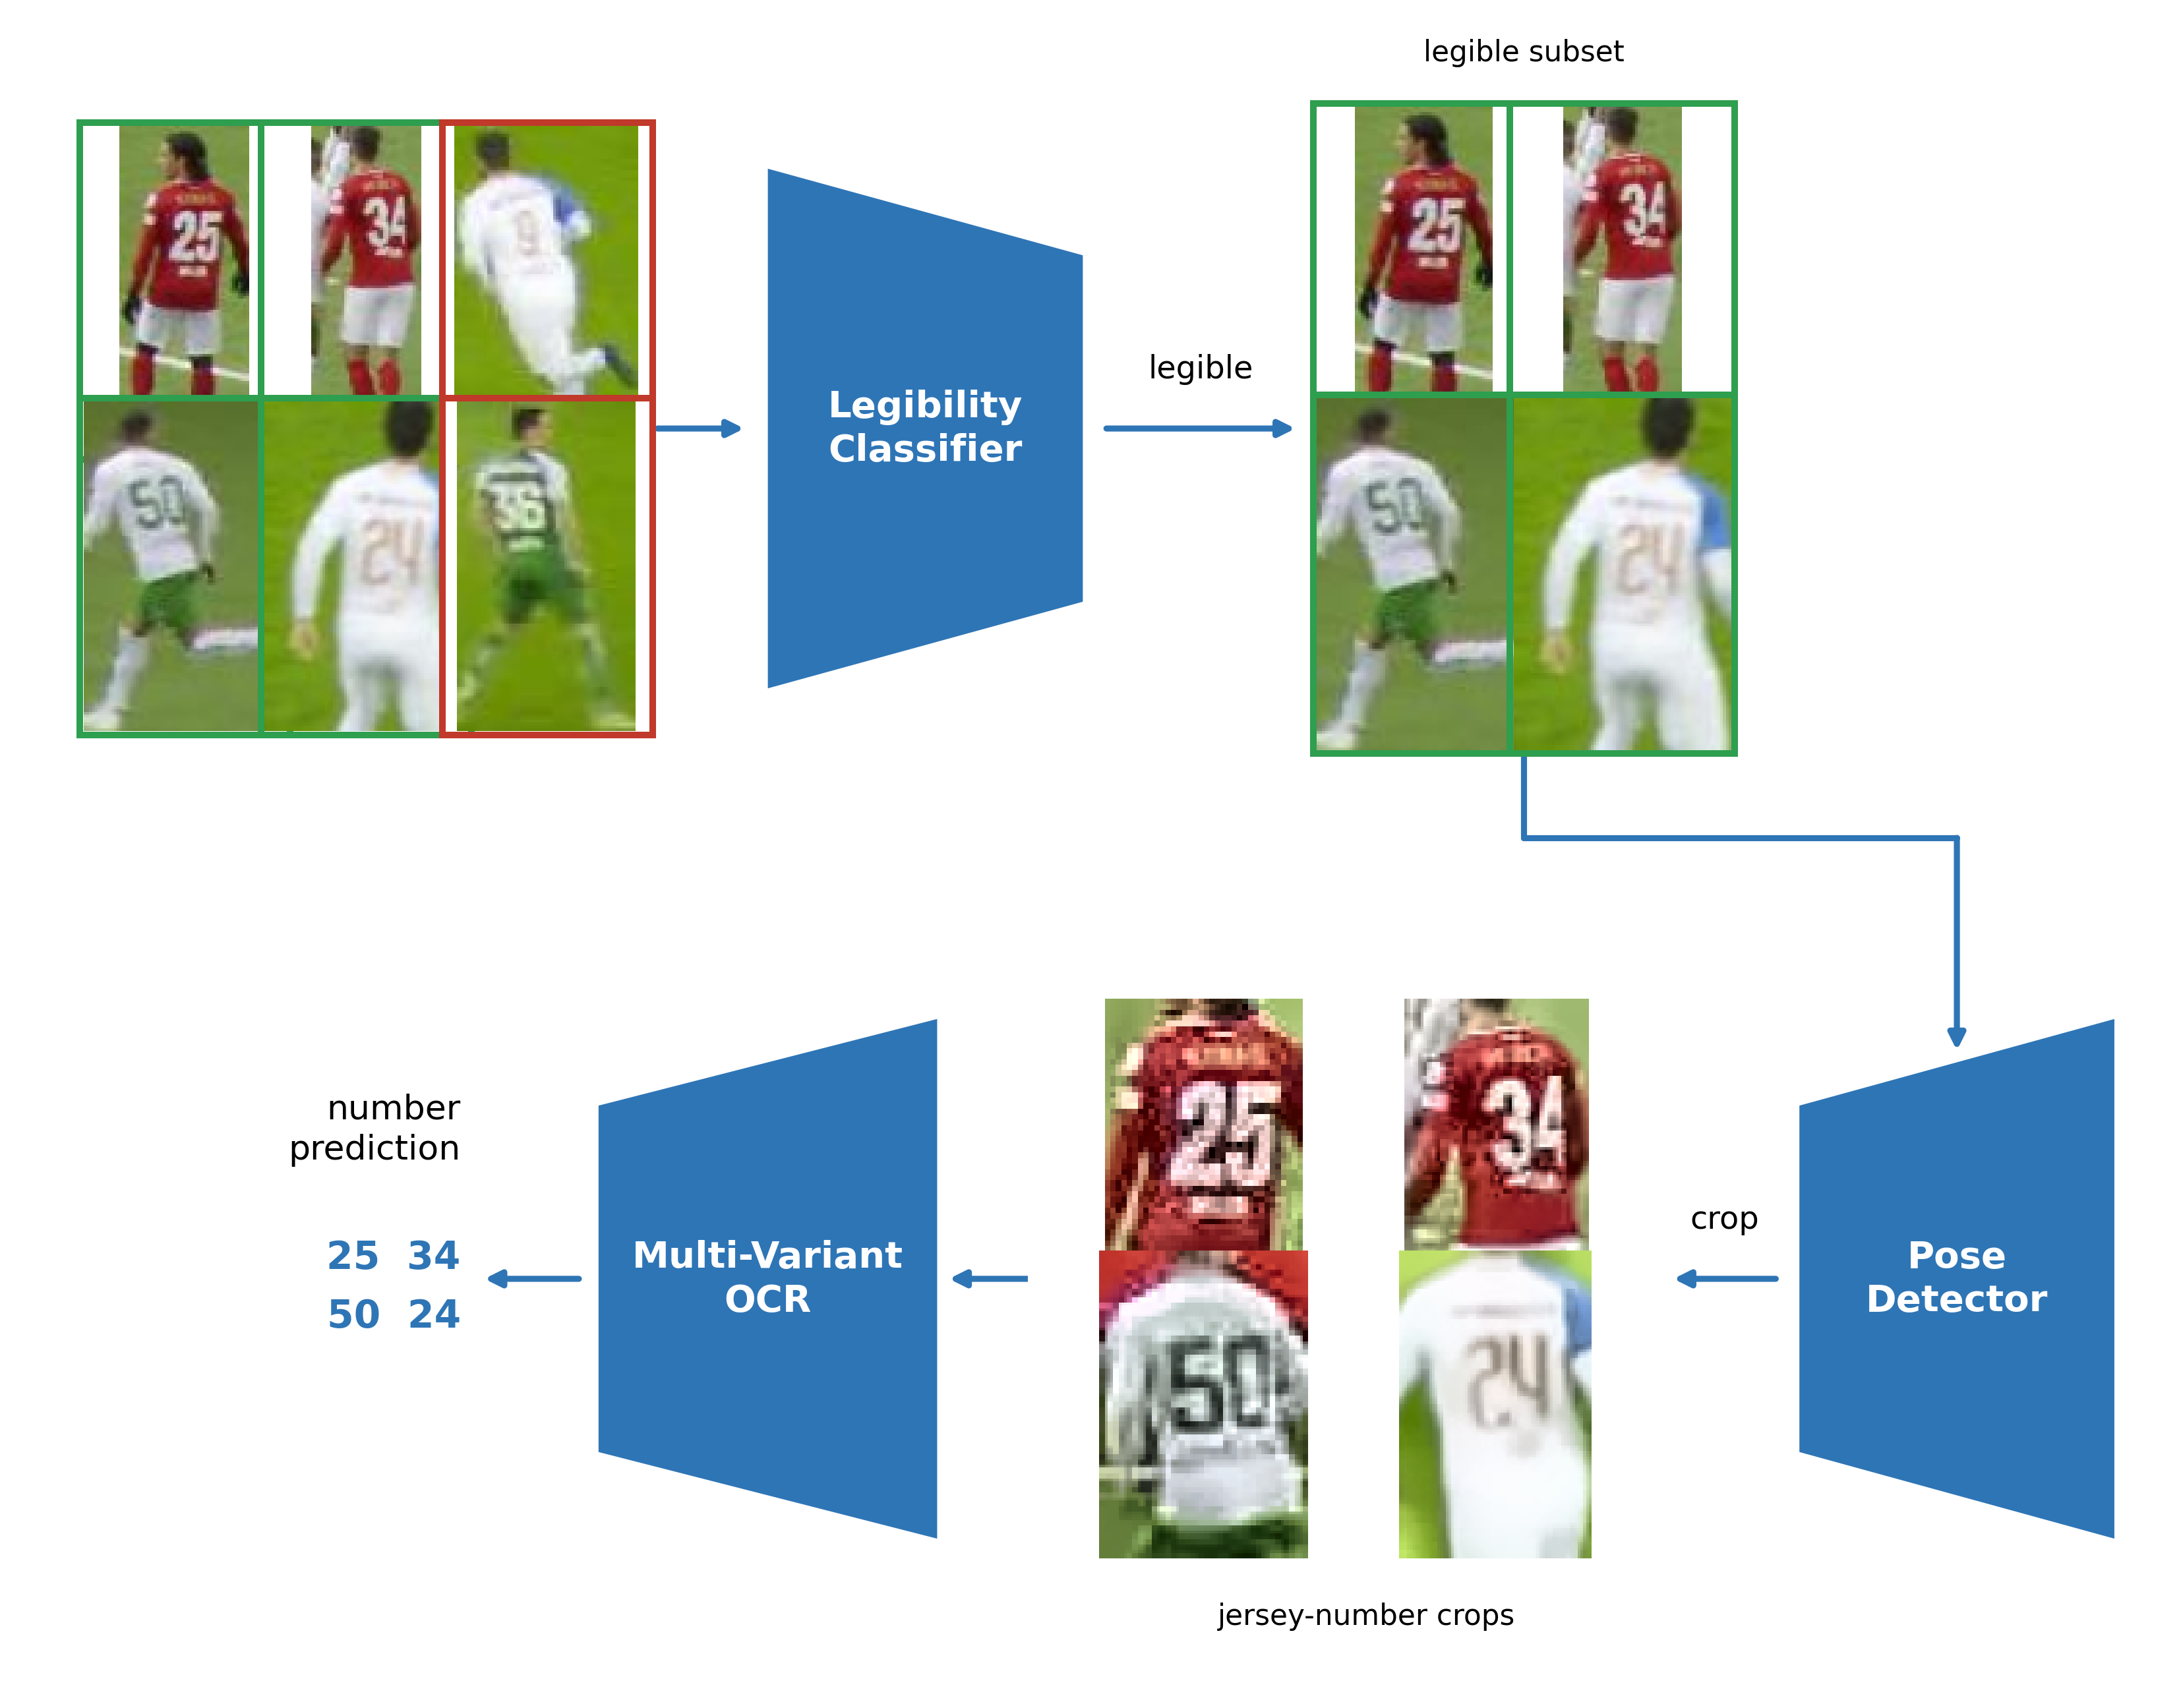
\includegraphics[width=\textwidth]{figures/fig_pipeline_reference_style.png}
    \caption{Reference-style overview of the image-based jersey number
    recognition pipeline. The pipeline progresses from raw player images
    through detection, pose-driven torso localization, image enhancement,
    and multi-variant OCR to a final per-player jersey number prediction.
    Each block represents a distinct processing module; arrows show the
    flow of image and metadata artefacts between them.}
    \label{fig:pipeline-reference}
\end{figure}

Figure~\ref{fig:image-pipeline-tikz} re-draws this pipeline as a
vertically stacked, phase-grouped process diagram to clarify the logical
grouping of stages.

\begin{figure}[H]
    \centering
    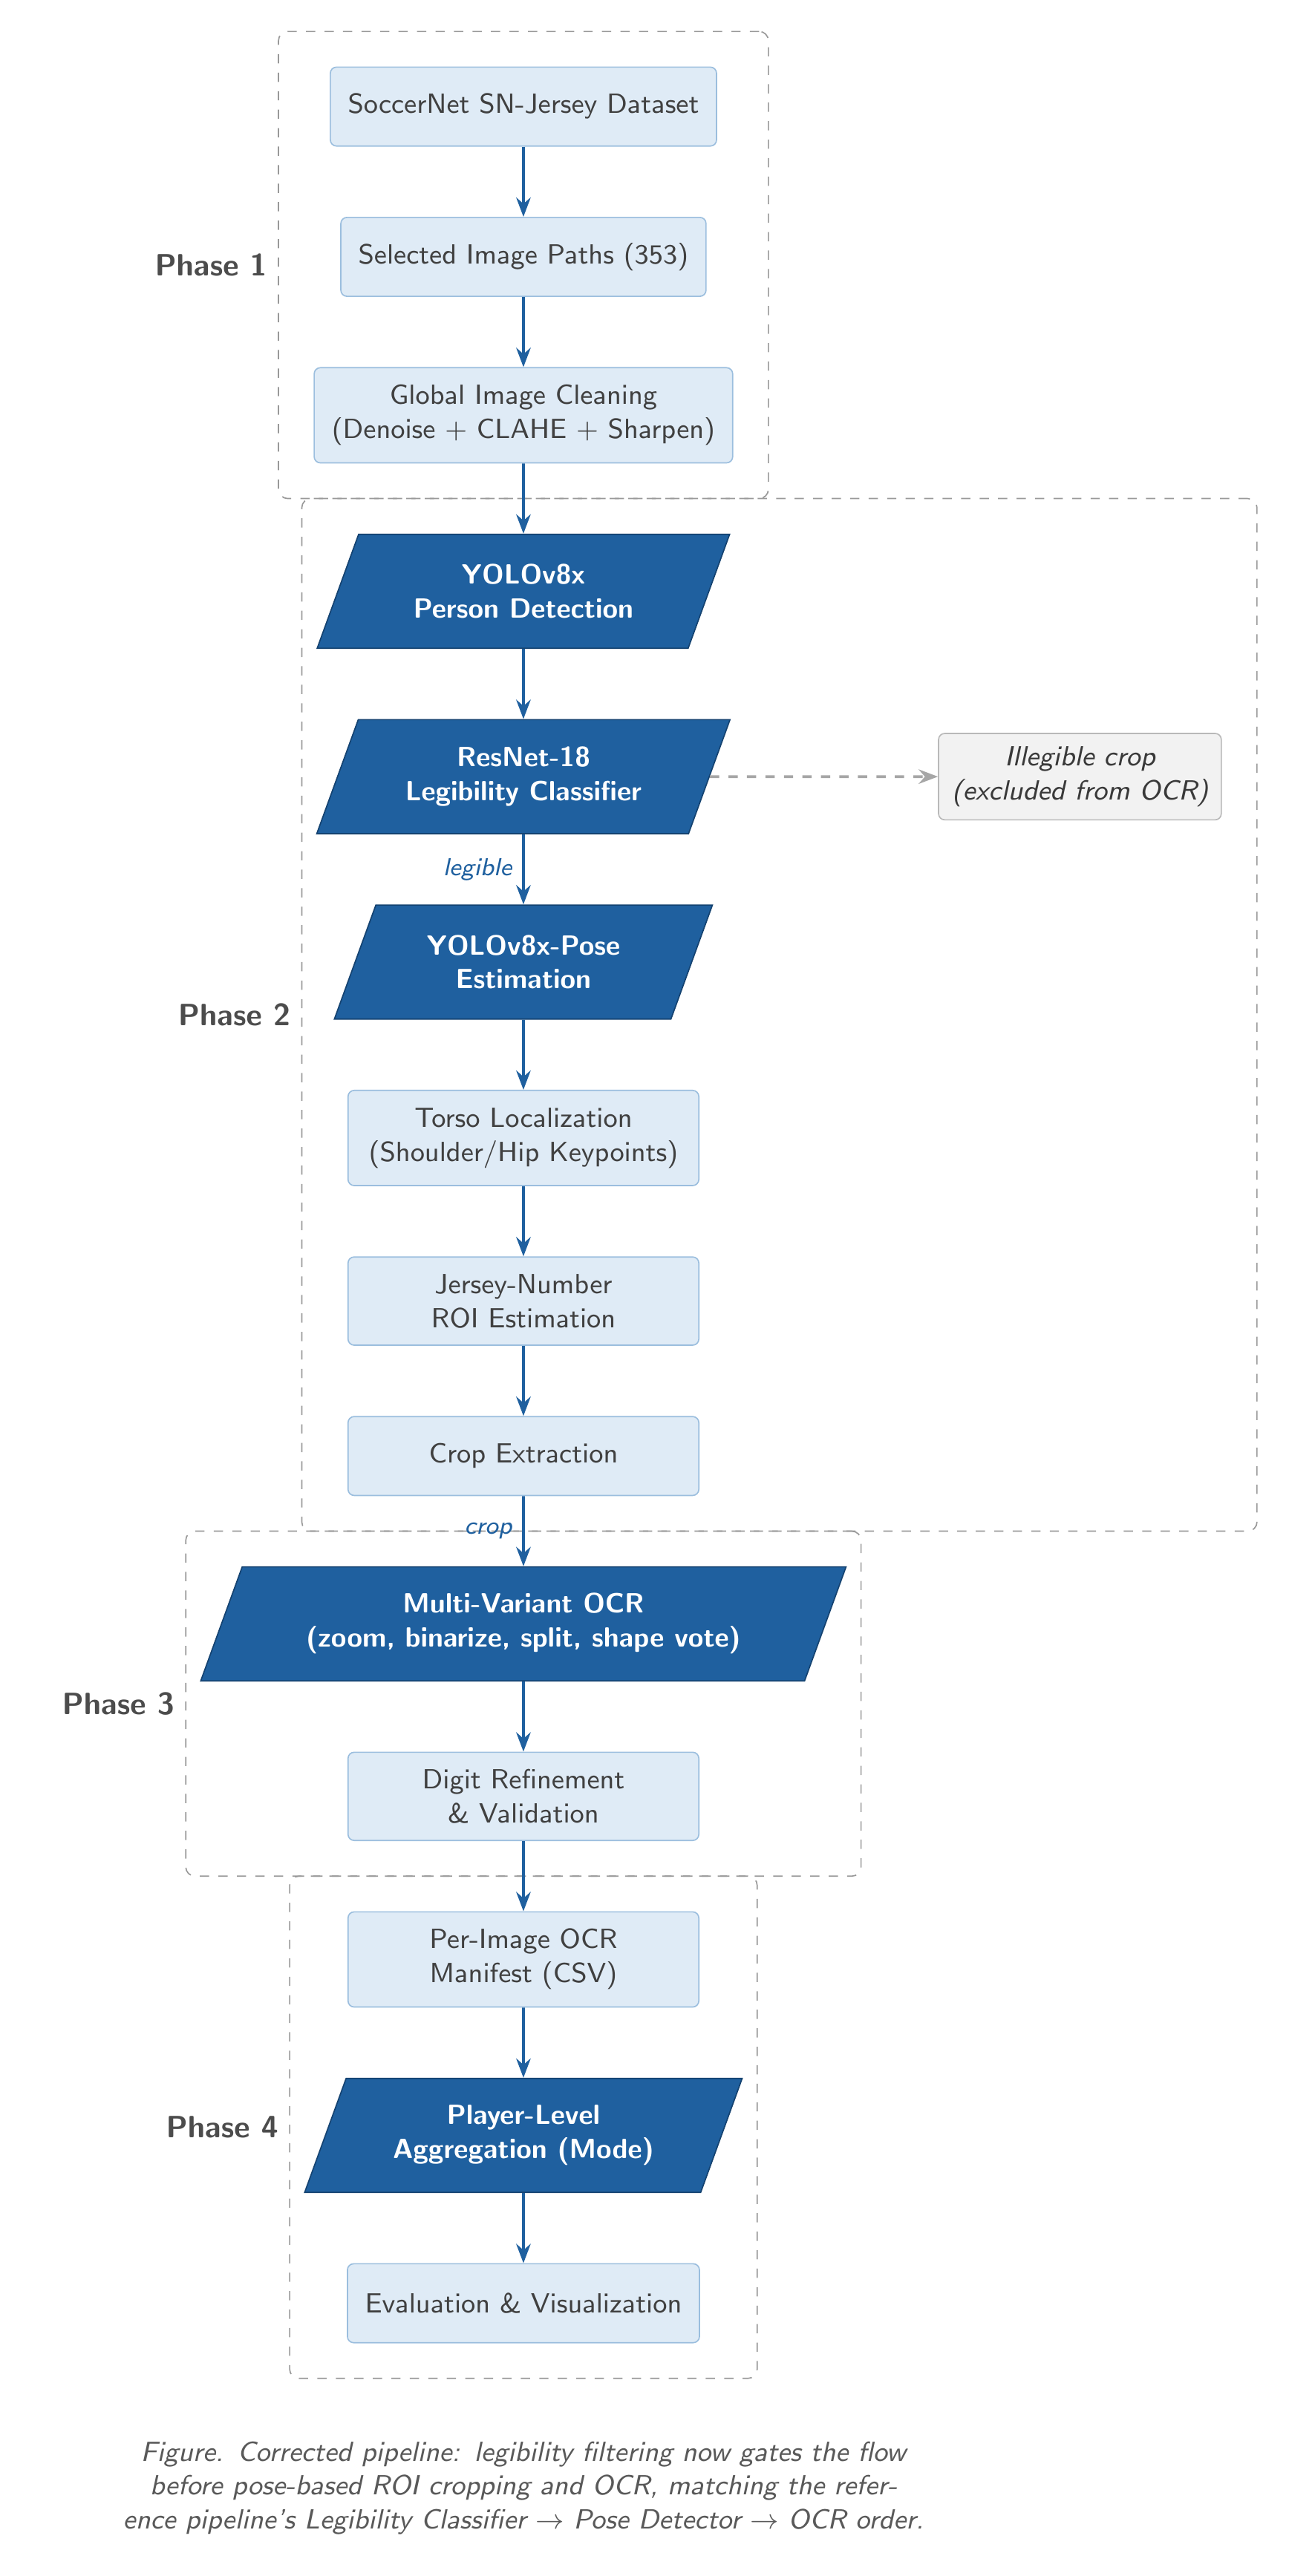
\includegraphics[width=0.72\textwidth]{figures/tikz_image_pipeline.png}
    \caption{Phase-grouped workflow of the image pipeline. Phase~1 handles data preparation. Phase~2 performs person detection followed by legibility classification, which filters out illegible crops before pose estimation and torso/ROI localization proceed on the remaining legible crops, yielding the final jersey-number crop. Phase~3 runs multi-variant OCR on these crops, followed by digit refinement and validation. Phase~4 aggregates per-crop OCR results into player-level predictions and evaluates them against ground truth.}
    \label{fig:image-pipeline-tikz}
\end{figure}

\subsection{Module Descriptions}

\paragraph{Data preparation.} The pipeline downloads the SoccerNet
SN-Jersey dataset and locates the \texttt{train}/\texttt{test} image
directories and ground-truth JSON files. A curated list of 353 image
paths parsed from \texttt{img\_path.txt} is decomposed into split,
player ID, and image ID for each entry. This curated selection ensures
a representative distribution of jersey numbers, image resolutions,
and lighting conditions, while remaining computationally tractable for
single-GPU execution.

\paragraph{Detection and torso localization.} Each image is first
enhanced by \texttt{clean\_main\_image()}. The \texttt{PlayerDetector}
(YOLOv8x) then locates person bounding boxes. Only
\mbox{\texttt{class\_id == 0}} (COCO \texttt{person}) detections with
confidence $\geq 0.20$ are retained. Next, the
\texttt{PoseHelper} (YOLOv8x-Pose) estimates 17 COCO body keypoints
per detection; shoulder keypoints (indices 5 and 6) and hip keypoints
(indices 11 and 12) are matched to player boxes via IoU. From these
keypoints, the torso bounding box is computed, and the jersey-number
region of interest (ROI) is derived by narrowing to the central
30--70\% (horizontal) and 20--80\% (vertical) of the torso box before
applying a proportional expansion margin of 18\% horizontal, 12\% top,
and 22\% bottom.

\paragraph{OCR and legibility.} Each crop is passed to
\texttt{ocr\_digits\_strict()} (Section~\ref{sec:multi-variant-ocr}),
which returns the best digit string, its confidence, and the method tag
used. The multi-variant OCR engine evaluates up to six enhancement
variants at four zoom scales, runs per-digit isolation with six
binarization strategies, performs projection-based digit splitting, and
applies shape-based digit disambiguation for the commonly confused digit
pairs (0/6/8/9 and 1/7). A separate stage derives weak legibility
labels from the OCR manifest and trains the ResNet-18
\texttt{LegibilityModel} for use as a pre-filter.

\paragraph{Aggregation and evaluation.} All per-crop results are
written to \texttt{crops\-\_ocr\-\_manifest.csv}. Player-level predictions
are obtained as the statistical \textbf{mode} of \texttt{best\-\_digits}
across all crops for each player --- effectively the jersey number that
the pipeline predicts most consistently for that player's images.
These mode predictions are compared against ground-truth numbers to
compute accuracy, player-level confusion matrices, and confidence
statistics.

\subsection{Legibility Classifier Training}
\label{sec:legibility-training}

The \texttt{LegibilityModel} (ResNet-18, single-logit output) is trained
for \textbf{20 epochs} with the following configuration:

\begin{itemize}[noitemsep]
    \item \textbf{Input:} $96 \times 96$ RGB, normalized with ImageNet
    mean/standard deviation.
    \item \textbf{Augmentation (train only):} Random color jitter
    (brightness/contrast, $p=0.5$) and random rotation ($\pm5^{\circ}$).
    \item \textbf{Loss:} \texttt{BCEWithLogitsLoss} with \texttt{pos\_weight}
    set to the ratio of negative to positive samples, correcting for
    the natural class imbalance in the dataset (legible crops far
    outnumber illegible ones).
    \item \textbf{Optimizer:} AdamW, learning rate $2\times10^{-4}$,
    weight decay $1\times10^{-4}$.
    \item \textbf{Scheduler:} \texttt{ReduceLROnPlateau} (factor 0.6,
    patience 2 epochs, monitored on validation loss), reducing the
    learning rate when improvement stalls.
    \item \textbf{Train/validation split:} Stratified 80\%/20\% split
    of training-set crops, random state 42.
    \item \textbf{Batch size:} 64.
\end{itemize}

{\sloppy The best checkpoint (by validation accuracy) is saved to
\texttt{legibility\-\_clas\-si\-fier.pth}.}

\section{Video-Based Pipeline}
\label{sec:video-pipeline}

\subsection{High-Level Workflow}

The video pipeline processes ten broadcast football clips
frame-by-frame, performing detection, tracking, role classification,
torso extraction, enhancement, OCR, and temporal jersey voting.
Figure~\ref{fig:video-architecture} shows the system architecture
diagram generated from the implementation.

\begin{figure}[H]
    \centering
    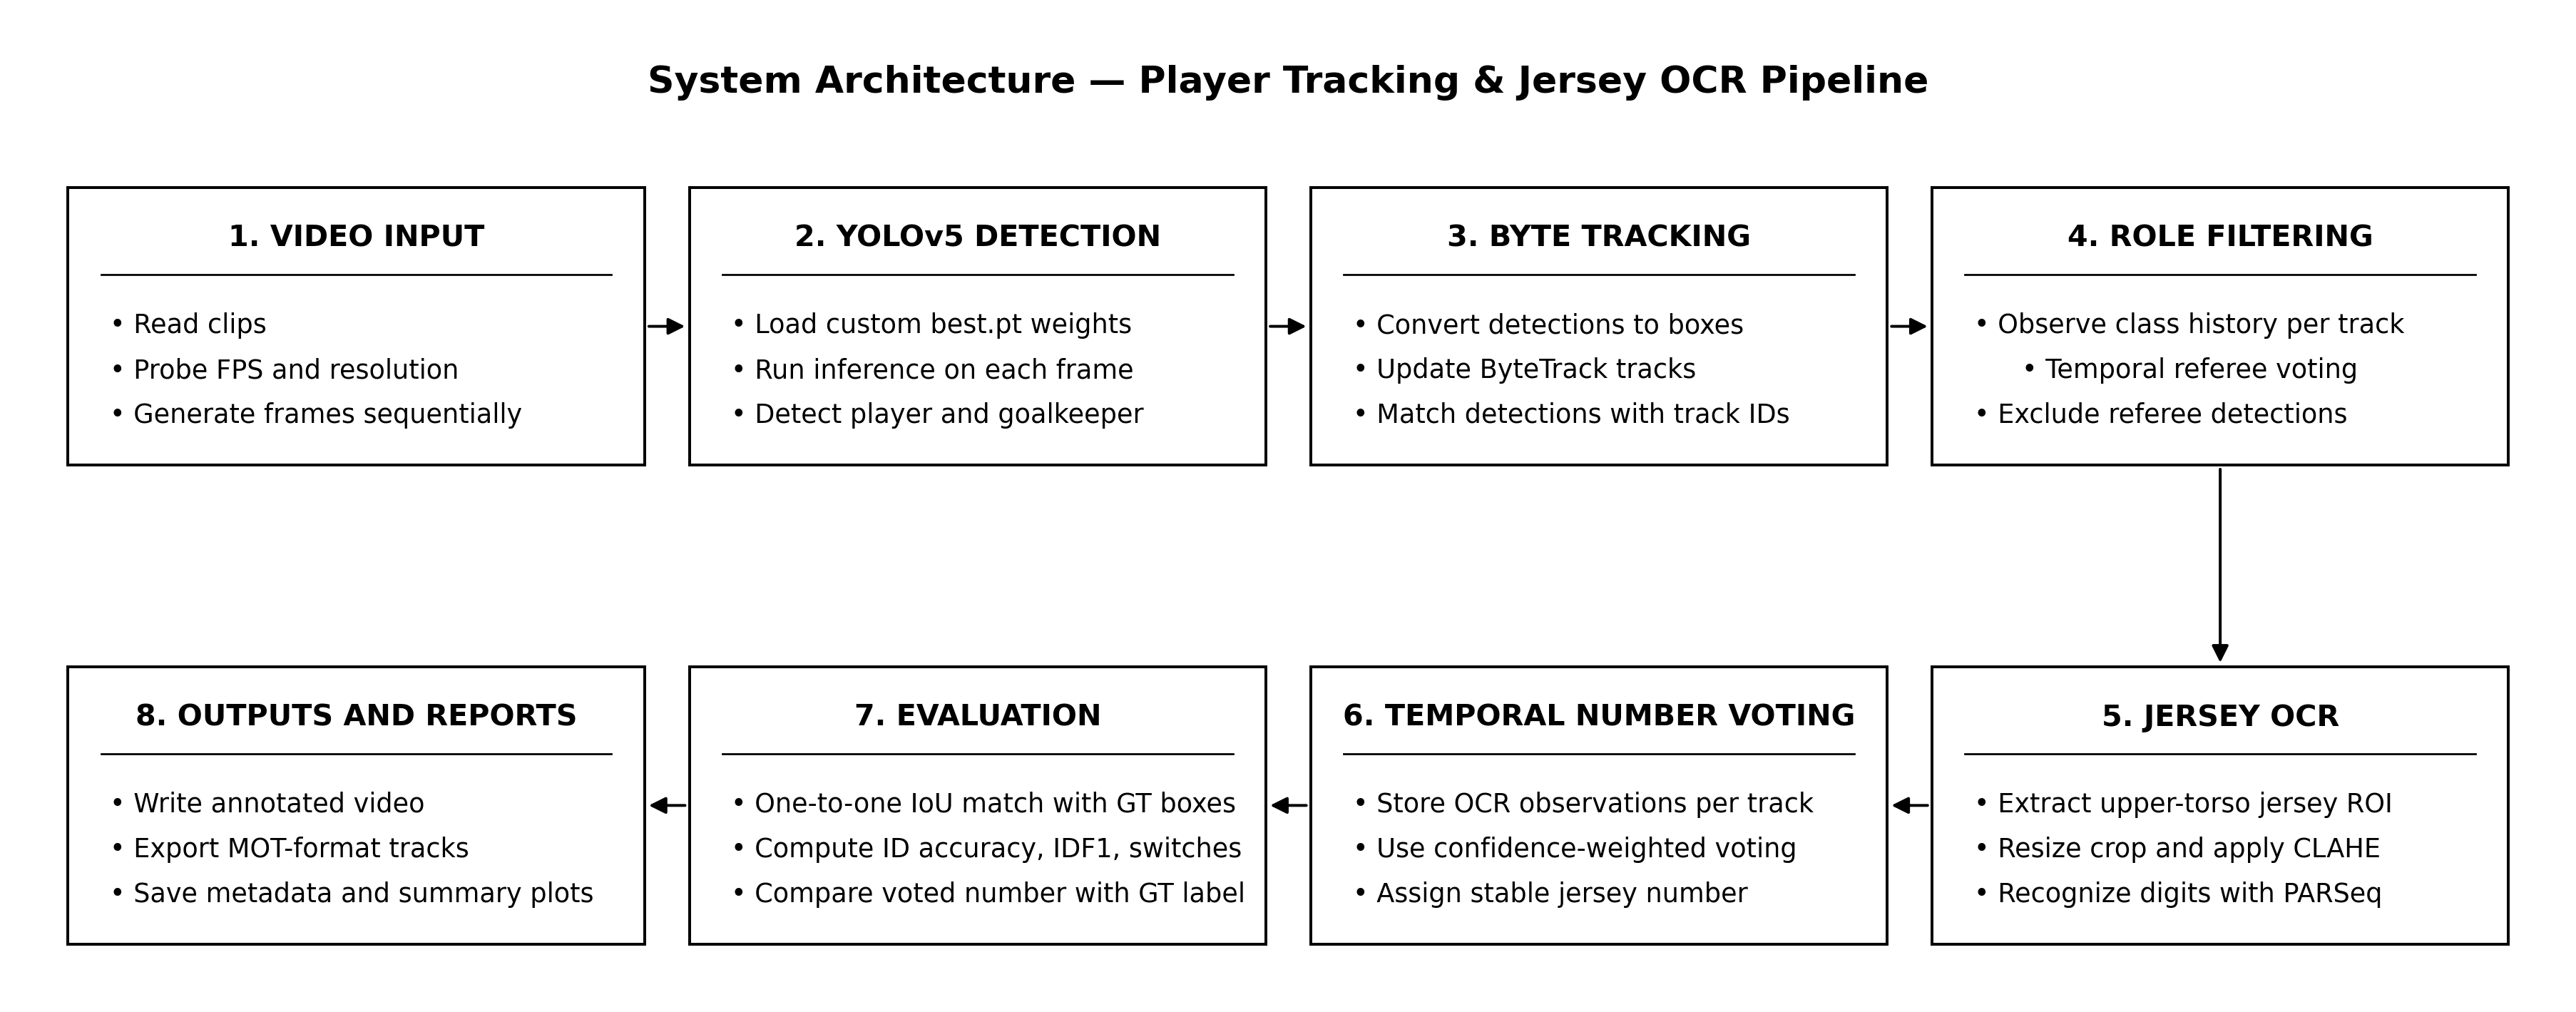
\includegraphics[width=1\textwidth]{figures/fig_video_architecture.png}
    \caption{System architecture of the video-based jersey number
    recognition pipeline. The architecture separates the frame-level
    processing loop (detection, tracking, role voting, torso extraction,
    OCR) from the post-processing evaluation stage (temporal jersey
    voting, ground-truth matching, metric computation).}
    \label{fig:video-architecture}
\end{figure}

Figure~\ref{fig:video-pipeline-diagram} shows the track-level jersey OCR
pipeline schematic, which explicitly illustrates how detections from the
YOLOv5 model flow through ByteTrack into per-track temporal voters.

\begin{figure}[H]
    \centering
    \includegraphics[width=\textwidth]{figures/fig_video_pipeline.png}
    \caption{Track-level jersey OCR pipeline diagram. Each detected
    player bounding box is first associated to a persistent track by
    ByteTrack; the torso region of that box is then enhanced and OCR'd.
    Per-frame results feed into the temporal jersey voter, which outputs
    a consensus jersey number per track once sufficient evidence has
    accumulated. At the end of each clip, the ground-truth evaluator
    matches predicted tracks to annotated tracks and computes both
    tracking and jersey recognition accuracy.}
    \label{fig:video-pipeline-diagram}
\end{figure}

Figure~\ref{fig:video-pipeline-tikz} presents a compact TikZ flowchart
that emphasizes the per-frame loop structure and the two output branches.

\begin{figure}[H]
    \centering
    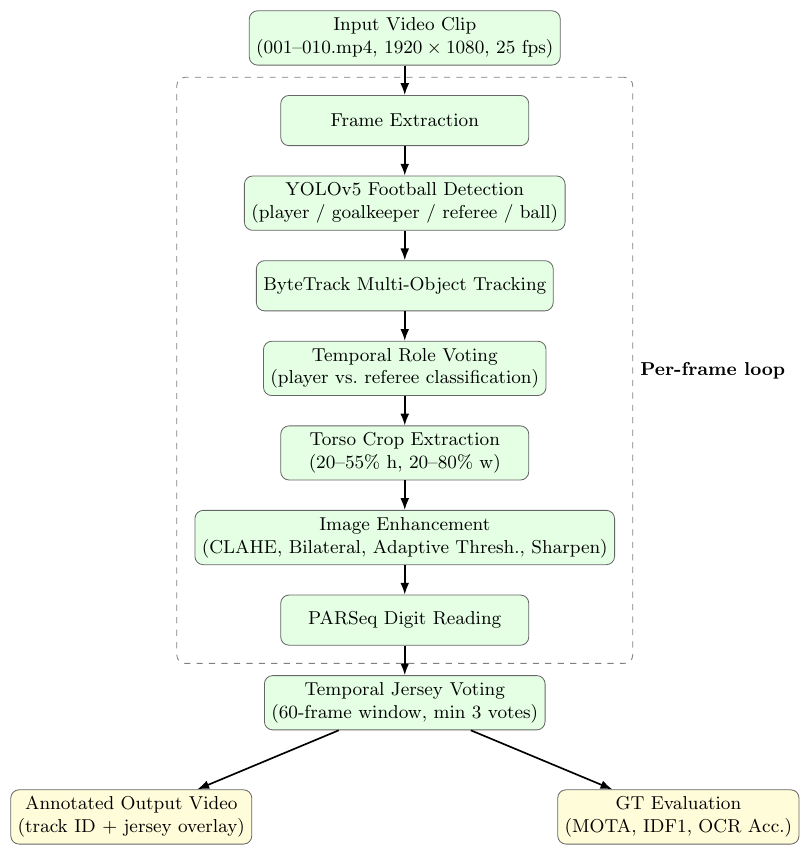
\includegraphics[width=0.72\textwidth]{figures/tikz_video_pipeline.png}
    \caption{Compact flowchart of the video pipeline, showing the
    per-frame processing loop and the two output branches:
    an annotated video and a ground-truth evaluation report.}
    \label{fig:video-pipeline-tikz}
\end{figure}

\subsection{Module Descriptions}

\paragraph{Detection.} For each frame, the YOLOv5 football model
(\texttt{model(frame,\allowbreak{} size=1280)}) produces bounding boxes for all
detected objects. The input frame is resized to 1280 pixels on the
longer side, preserving aspect ratio, before inference. Player and
goalkeeper detections are selected for tracking; ball detections are
discarded for the purpose of this pipeline.

\paragraph{Tracking.} The standalone ByteTrack implementation converts
player/goalkeeper detection boxes to its required $(x_1, y_1, x_2, y_2,
\text{conf})$ format using \texttt{detec\-tions2\-boxes()}, then updates the
Kalman-filter motion model and performs IoU-based frame-to-frame
association. The tracker maintains a \emph{lost} buffer of
\texttt{track\-\_buffer=30} frames, allowing temporarily occluded players
to be re-associated to their existing track ID rather than spawning a
new track.

\paragraph{Temporal role voting.} The \texttt{Temporal\-Role\-Voter}
maintains a per-track deque of the most recent 20 semantic class labels.
Once at least 5 observations are accumulated, if the referee class
constitutes $\geq 60\%$ of them, the track is permanently locked as
\textit{referee} and excluded from all subsequent OCR processing. This
avoids wasting OCR resources on match officials while also preventing
referee jersey numbers from polluting player records.

\paragraph{Torso extraction and enhancement.} For non-referee tracks,
\texttt{extract\-\_torso()} crops the region spanning 20--80\% of the
player box width and 20--55\% of the player box height, subject to a
minimum crop size of $30 \times 40$ pixels. If the crop is smaller than
$32 \times 64$ pixels, it is up-sampled using cubic interpolation. Four
enhancement variants are produced: CLAHE ($\texttt{clipLimit}=3.0$),
bilateral filter followed by CLAHE, adaptive thresholding with
morphological closing, and a $3\times3$ high-pass sharpening kernel.

\paragraph{OCR and temporal voting.} Each enhanced variant is passed
through the \texttt{JerseyRecognizer}, which attempts PARSeq first
(loaded via \texttt{torch.hub} from the \texttt{baudm/parseq}
repository) with \texttt{allowlist='0123456789'} and
\texttt{max\_candidates=2}, and falls back to EasyOCR with the same
allowlist if PARSeq is unavailable in the runtime environment. Valid
jersey numbers (1--2 digits, integer value in $[1, 99]$) with
confidence $\geq 0.25$ are fed into the \texttt{Temporal\-Jersey\-Voter}.
The voter returns the plurality jersey number within the 60-frame
window once at least 3 valid votes have been accumulated.

\paragraph{Ground-truth evaluation.} After all clips are processed,
the \texttt{GT\-Tracking\-And\-Jersey\-Evaluator} loads per-video MOT
ground-truth files (providing per-frame player bounding-box positions
and track IDs) and jersey-number CSV files (providing manually annotated
jersey numbers for a subset of tracks). Predicted and ground-truth
tracks are matched frame-by-frame using an IoU threshold of 0.30.
Standard MOT metrics --- tracking accuracy (equivalent to MOTA), IDF1,
ID precision, track recall, and ID switches --- are computed alongside
OCR accuracy.

\paragraph{Output.} Each clip produces: (a) an annotated output video
with bounding boxes, track IDs, and jersey number overlays; (b) a
per-video JSON metadata file; and (c) summary CSVs and figures exported
to the \texttt{reports/} directory.

\section{Comparison of the Two Pipeline Designs}

Table~\ref{tab:pipeline-comparison} summarizes the key architectural
differences between the two pipelines.

\begin{table}[H]
    \centering
    \caption{Comparison of the image-based and video-based pipeline designs.}
    \label{tab:pipeline-comparison}
    \resizebox{\textwidth}{!}{%
    \begin{tabular}{@{}p{3.4cm}p{5.0cm}p{5.0cm}@{}}
        \toprule
        \textbf{Aspect} & \textbf{Image Pipeline} & \textbf{Video Pipeline} \\
        \midrule
        Input & SoccerNet SN-Jersey crops (353 images) & 10 broadcast clips (900 frames each, $1920\times1080$) \\
        Detection model & YOLOv8x (generic person detector) & YOLOv5 (football-specific: player/goalkeeper/referee/ball) \\
        Player localization & YOLOv8x + YOLOv8x-Pose torso keypoints & YOLOv5 detection (no pose) \\
        Tracking & Not required (identity from folder structure) & ByteTrack persistent track ID \\
        Torso ROI & Pose-driven keypoint-based torso $\rightarrow$ ROI & Fixed-fraction heuristic (20--55\% h, 20--80\% w) \\
        OCR strategy & Multi-variant + zoom + per-digit isolation + shape vote (EasyOCR) & Four-variant PARSeq with EasyOCR fallback and validity filter \\
        Aggregation & Per-player mode over all crops & Temporal jersey voting (60-frame window) \\
        Legibility filter & Dedicated ResNet-18 classifier & Min crop height threshold only \\
        Referee handling & Not explicitly filtered & Temporal role voter (semantic class labels) \\
        Ground truth & Yes (SoccerNet \texttt{*\_gt.json}) & Yes (MOT GT files + jersey CSV files) \\
        \bottomrule
    \end{tabular}}
\end{table}

\section{Software Environment}
\label{sec:software-env}

Table~\ref{tab:software-stack} lists the key libraries and tools used
across both pipelines.

\begin{table}[H]
    \centering
    \caption{Software stack and libraries used in this thesis.}
    \label{tab:software-stack}
    \begin{tabular}{@{}ll@{}}
        \toprule
        \textbf{Component} & \textbf{Library / Tool} \\
        \midrule
        Deep learning framework & PyTorch, Torchvision \\
        Object detection (image) & Ultralytics YOLOv8 (\texttt{yolov8x.pt}, \texttt{yolov8x-pose.pt}) \\
        Object detection (video) & YOLOv5 football-specific model \\
        Multi-object tracking & ByteTrack (standalone Python implementation) \\
        OCR engine (image) & EasyOCR (multi-variant digit recognizer) \\
        OCR engine (video) & PARSeq (\texttt{baudm/parseq}), EasyOCR fallback \\
        Image processing & OpenCV (\texttt{cv2}), Pillow (PIL) \\
        Data handling & NumPy, Pandas \\
        Visualization & Matplotlib, Seaborn \\
        Evaluation & scikit-learn (confusion matrix, PR/ROC curves) \\
        Dataset access & SoccerNet Python package \\
        Execution environment & Kaggle (GPU runtime, NVIDIA P100) \\
        \bottomrule
    \end{tabular}
\end{table}
